% !TEX TS-program = pdflatexmk
\documentclass[12pt]{article}

% Layout.
\usepackage[top=1in, bottom=0.75in, left=1in, right=1in, headheight=1in, headsep=6pt]{geometry}

% Fonts.
\usepackage{mathptmx}
\usepackage[scaled=0.86]{helvet}
\renewcommand{\emph}[1]{\textsf{\textbf{#1}}}

% TiKZ.
\usepackage{tikz, pgfplots}
\usetikzlibrary{calc}
\pgfplotsset{my style/.append style={axis x line=middle, axis y line=
middle, xlabel={$x$}, ylabel={$y$}, axis equal }}

% Misc packages.
\usepackage{amsmath,amssymb,latexsym}
\usepackage{graphicx}
\usepackage{array}
\usepackage{xcolor}
\usepackage{multicol}

% Commands to set various header/footer components.
\makeatletter
\def\doctitle#1{\gdef\@doctitle{#1}}
\doctitle{Use {\tt\textbackslash doctitle\{MY LABEL\}}.}
\def\docdate#1{\gdef\@docdate{#1}}
\docdate{Use {\tt\textbackslash docdate\{MY DATE\}}.}
\def\doccourse#1{\gdef\@doccourse{#1}}
\let\@doccourse\@empty
\def\docscoring#1{\gdef\@docscoring{#1}}
\let\@docscoring\@empty
\def\docversion#1{\gdef\@docversion{#1}}
\let\@docversion\@empty
\makeatother

% Headers and footers layout.
\makeatletter
\usepackage{fancyhdr}
\pagestyle{fancy}
\fancyhf{} % Clears all headers/footers.
\lhead{\baselineskip 30pt
\emph{\@doctitle\hfill\@docdate}
\ifnum \value{page} > 1\relax\else\\
\emph{Name: \rule{3.5in}{1pt}\hfill \@docscoring}\fi}
\rfoot{\emph{\@docversion}}
\lfoot{\emph{\@doccourse}}
\cfoot{\emph{\thepage}}
\renewcommand{\headrulewidth}{0pt}%
\makeatother

% Paragraph spacing
\parindent 0pt
\parskip 6pt plus 1pt

% A problem is a section-like command. Use \problem{5} to
% start a problem worth 5 points.
\newcounter{probcount}
\newcounter{subprobcount}
\setcounter{probcount}{0}
\newcommand{\problem}[1]{%
\par
\addvspace{4pt}%
\setcounter{subprobcount}{0}%
\stepcounter{probcount}%
\makebox[0pt][r]{\emph{\arabic{probcount}.}\hskip1ex}\emph{[#1 points]}\hskip1ex}
\newcommand{\thesubproblem}{\emph{\alph{subprobcount}.}}

% Subproblems are an enumerate-like environment with a consistent
% numbering scheme. 
% Use \begin{subproblems}\item...\item...\end{subproblems}
\newenvironment{subproblems}{%
\begin{enumerate}%
\setcounter{enumi}{\value{subprobcount}}%
\renewcommand{\theenumi}{\emph{\alph{enumi}}}}%
{\setcounter{subprobcount}{\value{enumi}}\end{enumerate}}

% Blanks for answers in normal and math mode.
\newcommand{\blank}[1]{\rule{#1}{0.75pt}}
\newcommand{\mblank}[1]{\underline{\hspace{#1}}}
\def\emptybox(#1,#2){\framebox{\parbox[c][#2]{#1}{\rule{0pt}{0pt}}}}

% Misc.
\renewcommand{\d}{\displaystyle}
\newcommand{\ds}{\displaystyle}
\def\bc{\begin{center}}
\def\ec{\end{center}}


\doctitle{Math 251: Quiz 6}
\docdate{Oct 22, 2019}
\doccourse{UAF Calculus I}
\docversion{v-2}
\docscoring{\blank{0.8in} / 25}
\begin{document}
There are 25 points possible on this quiz. No aids (book, calculator, etc.)
are permitted.  Show all work for full credit.

%velocity & acceleration
\problem{8} A small bug is crawling along a branch of a tree. The bug's distance, in millimeters, from the trunk after $t$ seconds is given by the function
$$s(t)=6t-\frac{9}{2}t^2+t^3.$$
	\begin{subproblems}
	\item What is the velocity of the bug at time $t$?
	\vfill
	\item When is the bug at rest?
	\vfill
	\item What is the acceleration of the bug when it's at rest?
	\vfill
	\item At time $t=3$, is the bug moving toward the trunk or away from the trunk? Justify your answer.
	\vfill
	\end{subproblems}
\problem{2} Let $P$ denote the population of an invasive species of fish that is growing over time, $t$. Suppose the population $P$ grows at a rate proportional its size. What can you say about the function $P(t)$?
\vspace{2in}
\newpage
%Linearization\differentials
\problem{6} The edge of a cube was found to be 5 meters with a possible error in measurement of 0.1 meter. Use differentials to estimate the maximum possible error in computing the surface area of the cube. Include units with your answer.
\vfill
%related rate
\problem{9} The altitude (height, $h$) of a triangle is increasing at at rate of 3 cm/sec while the area of the triangle is decreasing at a rate of 1 $\text{cm}^2$/sec. At what rate is the base, $b$, of the triangle changing with the altitude is 20 cm and the area is 100 $\text{cm}^2$? Include units with your answer.

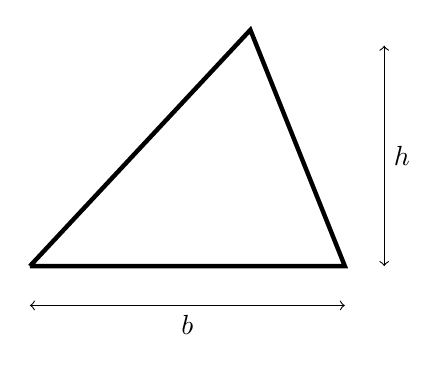
\begin{tikzpicture}
\draw[ultra thick] (0,0)--(4,0)--(2.8,3)--(0,0);
\draw[<->] (0,-.5)-- node[below]{$b$}  (4,-.5);
\draw[<->] (4.5,0)-- node[right]{$h$}  (4.5,2.8);
\end{tikzpicture}
\vspace{4in}


%\problem{2} A population of voles has an initial population of 10 voles. One year later the population is 23 voles. Assume that this populations grows at a rate proportional to its size. 
%	\begin{subproblems}
%	\item Find an expression for the number of voles after $t$ years.\\
%	\vfill
%	\item Determine when the population will reach 1000 voles.\\
%	\vfill
%	\end{subproblems}
\end{document}



